\documentclass[8pt, sans]{beamer}
\usepackage{etex}
\usepackage{enumitem}
%\reserveinserts{28}
\usepackage{amssymb}
\usepackage{theorem}
%\usepackage{savetrees}
%\usepackage[margin=2cm]{geometry}
\usepackage{graphicx}
\usepackage{fancybox}
\usepackage{fancyhdr}
\usepackage{tabularx}
\usepackage{color}
\usepackage{xcolor}
\usepackage{multirow}
\usepackage{amsmath}
\usepackage[utf8]{inputenc} % Pour pouvoir taper les accent directement et non pas passer par \'
\usepackage[T1]{fontenc} %%% Pour que les accents soient correctement traités dans le PDF et le DVI
\usepackage{lmodern} %Un autre package pour les accents français
\usepackage[french]{babel} %Un autre package pour les accents
\usepackage{ifthen}
%\usepackage{multicol}
%\usepackage{cancel}
\usepackage{pst-all}
\usepackage{pstricks-add}
\usepackage{multicol}
%\usepackage{tikz}
%\usepackage{pgf,tikz}
%\usepackage{circuitikz}
%\usetikzlibrary{shapes}
%\usetikzlibrary{calc}
%\usetikzlibrary{plotmarks}
%\usepackage{tkz-fct}
\usepackage{fp}
\usepackage{float}
%\usepackage{siunitx}
\usepackage{pdfpages}%Pour sortir seulement certaine pages du pdf
\usepackage{textcomp}
\usepackage{hyperref}
%\hypersetup{
%    colorlinks=true, % make the links colored
%    linkcolor=blue, % color TOC links in blue
%    urlcolor=red, % color URLs in red
%    linktoc=all % 'all' will create links for everything in the TOC
%}

%\sisetup{locale = FR, number-math-rm, per-mode=symbol, separate-uncertainty}

\renewcommand{\exp}[1]{\mathrm{e}^{#1}}

%\setlength{\parindent}{0pt}


\begin{document}

\title{Les bandits stochastiques à récompenses d'espérance non-définie}
\author{Adam Cohen, Maxime Genest, Vincent Masse}
\maketitle

\begin{frame}
\frametitle{Rappel sur les bandits stochastiques classiques}
%\framesubtitle{Et son sous-titre}

\begin{itemize}

\item[$\bullet$] Ensemble de $K$ actions (bras, machines).

\item[$\bullet$] Chaque action $k$ est associée à un paramètre inconnu $\mu_k$ tel que $X_{k_t} \sim \nu\left(\mu_k\right)$ où $\nu\left(\mu_k\right)$ est une distribution d'espérance $\mu_k.$

\end{itemize}

\vfill

\pause

Dans le jeu des bandits stochastiques, à chaque pas de temps $t=1,2,\ldots,T,$ l'agent:

\begin{itemize}

\item[$\bullet$] Sélectionne une action $k_t\in\left\{1,2,\ldots K\right\}$ 

\item[$\bullet$] On observe une récompense (reward) $r_t\sim \nu\left(\mu_{k_t}\right).$

\end{itemize}

But: Déterminer une politique d'action qui maximisera $\displaystyle \mathbb{E}\left[\sum_{t=1}^T r_t\right]$\\

\vfill
\end{frame}


\begin{frame}
\frametitle{Mesure de performance empirique pour les bandits stochastiques}
Dans cette situation, à chaque pas de temps $t=1,2,\ldots,T,$ l'agent cumule un regret:

$$\Delta_{k_t}=\mu^{\star}-\mu_{k_t}$$ 
 
À la fin de l'épisode, on peut calculer le regret cumulatif empirique:

$$R(T)=\sum_{t=1}^T \Delta_{k_t}$$

Cela nous permet de comparer empiriquement la performance de plusieurs politiques, en simulant plusieurs épisodes et en comparant le regret cumulatif moyen sur ces épisodes.  

\end{frame}

\begin{frame}
\frametitle{L'hypothèse d'existence de l'espérance}
Le jeu des bandits stochastiques ainsi présenté sous-entend que la distribution des rewards associés aux bras du bandit est d'espérance qui existe. Or, plusieurs distributions de probabilité ont une distribution d'espérance non-définie. 

\pause
\vfill

Par exemple, La loi de Cauchy ou certaines configuration de la loi de Pareto.

\pause
\vfill
\textbf{Mettre des graphiques pour jaser un peu des queues des distribution}

\end{frame}

\begin{frame}
\frametitle{La loi de Cauchy}
La loi de Cauchy est une loi continue de fonction de densité 

$$f(x;L;a)=\frac{1}{\pi\,a\left[1+\left(\frac{x-L}{a}\right)^2\right]}=\frac{1}{\pi}\left[\frac{a}{(x-L)^2+a^2}\right]$$

où $l\in\mathbb{R}$ est un paramètre de localisation et $a>0$ est un paramètre d'échelle.

\pause

\begin{figure}[H]
\begin{center}
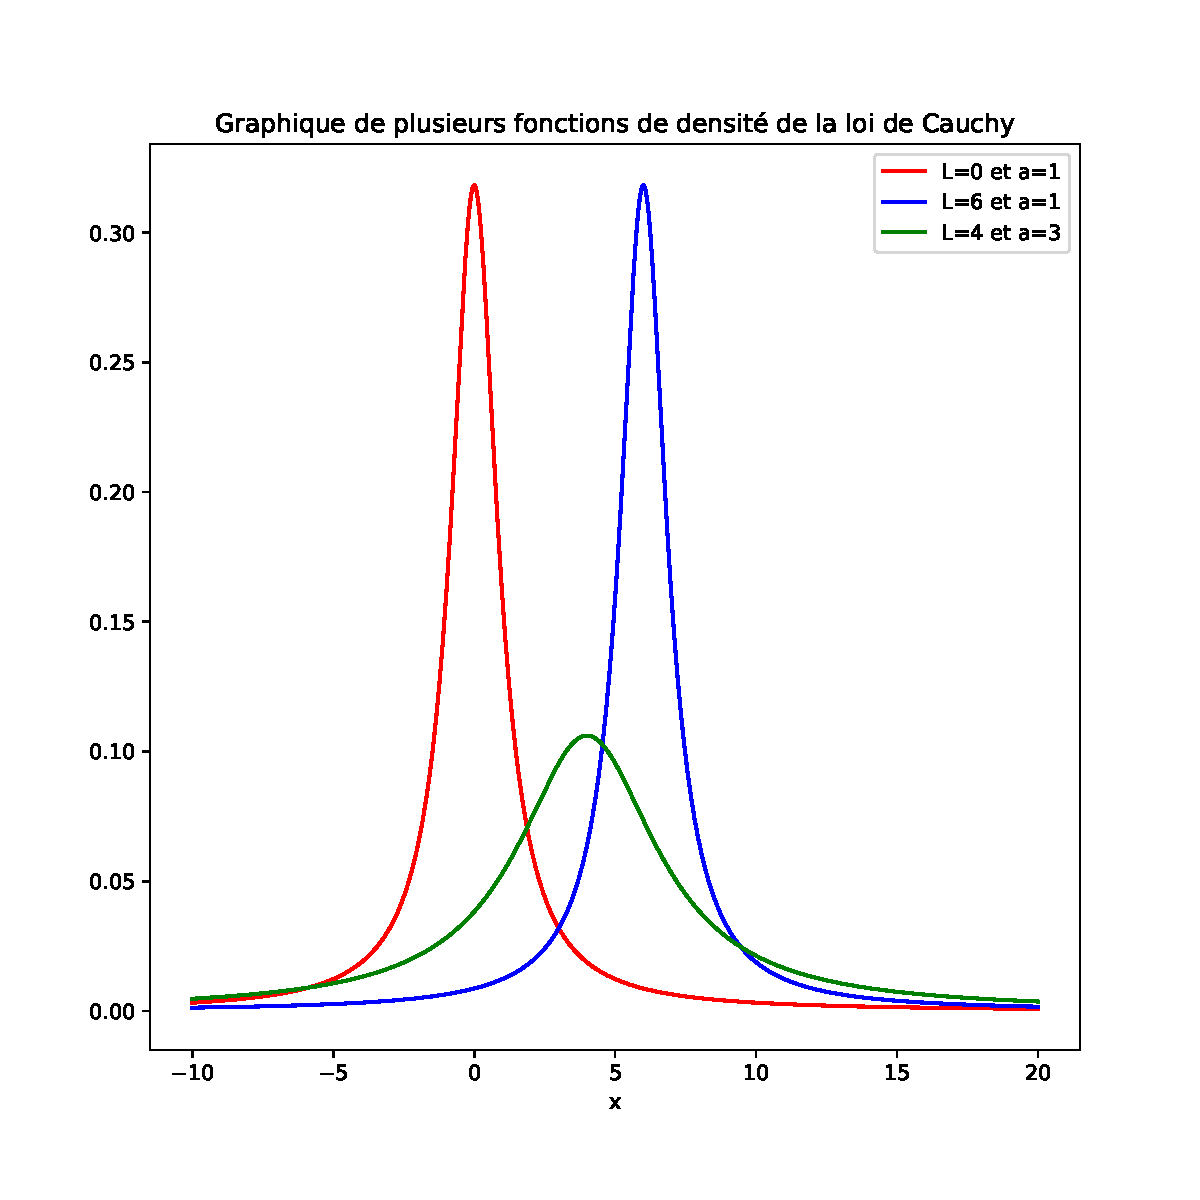
\includegraphics[scale=0.3]{graphiques_Cauchy.pdf}
\end{center}
\end{figure}

\end{frame}

\begin{frame}

\frametitle{Les bandits de Cauchy}

À chaque pas de temps $t=1,2,\ldots,T,$ l'agent:

\begin{itemize}

\item[$\bullet$] Sélectionne une action $k_t\in\left\{1,2,\ldots,K\right\}$

\item[$\bullet$] Observe une reward $r_t\sim \mathrm{Cauchy}(L_{k_t},a)$

\end{itemize}

\vfill
\pause

L'action optimale et la localisation optimale sont définis à partir de la localisation des différents bras:

\pause
$$\displaystyle L^{\star} := \max_k L_k \qquad \text{et} \qquad k^{\star} := \underset{k}{\mathrm{argmax}} L_k$$ 

\pause
\vfill

le gap (regret) associé à l'action $k$ devient $\Delta_k= L^{\star}-L_k$ 

\pause
\vfill

Mesure de performance empirique d'un agent: $\displaystyle R(T)=\sum_{t=1}^T \Delta_{k_t}$

\end{frame}

\begin{frame}
\frametitle{Les algorithmes classiques}

À faire: Montrer le graphique du regret d'une expérience basée sur un exemple d'algorithme classique basé sur la moyenne empirique 
\vfill
\pause

Cause de la mauvaise performance: la moyenne empirique $\hat \mu_k(t)$ n'est pas un bon estimateur de la localisation $L_k$ de la loi de Cauchy du bras no $k.$\\

\vfill
\pause

À faire, montrer une expérience montrant le comportement chaotique de l'estimateur $\hat \mu_{k}(t).$ 
\vfill

\end{frame}

\begin{frame}
\frametitle{Estimateurs de la localisation $L$ d'une loi de Cauchy}
Présentation des différents estimateurs de localisation pour le paramètre L

\end{frame}

\begin{frame}
\frametitle{Adaptation des algorithmes}
Présentation des différentes adaptations des algorithmes (etc, epsilon\_greedy,...) pour les bandits Cauchy.
\end{frame}

\begin{frame}
\frametitle{La loi de Pareto}
La loi de Pareto est une loi continue dont la fonction de densité est donnée par

$$f(x;x_m,k)=\left\{
\begin{array}{ll}
\dfrac{kx_m^k}{x^{k+1}} & \text{si $x\geq x_m$}\\
0                       & \text{sinon}
\end{array}
\right.
$$

Dans le cas particulier où $k=1$, on obtient que 

$$f(x;x_m)=\left\{
\begin{array}{ll}
\dfrac{x_m}{x^{2}} & \text{si $x\geq x_m$}\\
0                       & \text{sinon}
\end{array}
\right.
$$

Dans ce cas particulier, la loi de Pareto possède une espérance non-définie (infinie).

\begin{figure}[H]
\begin{center}
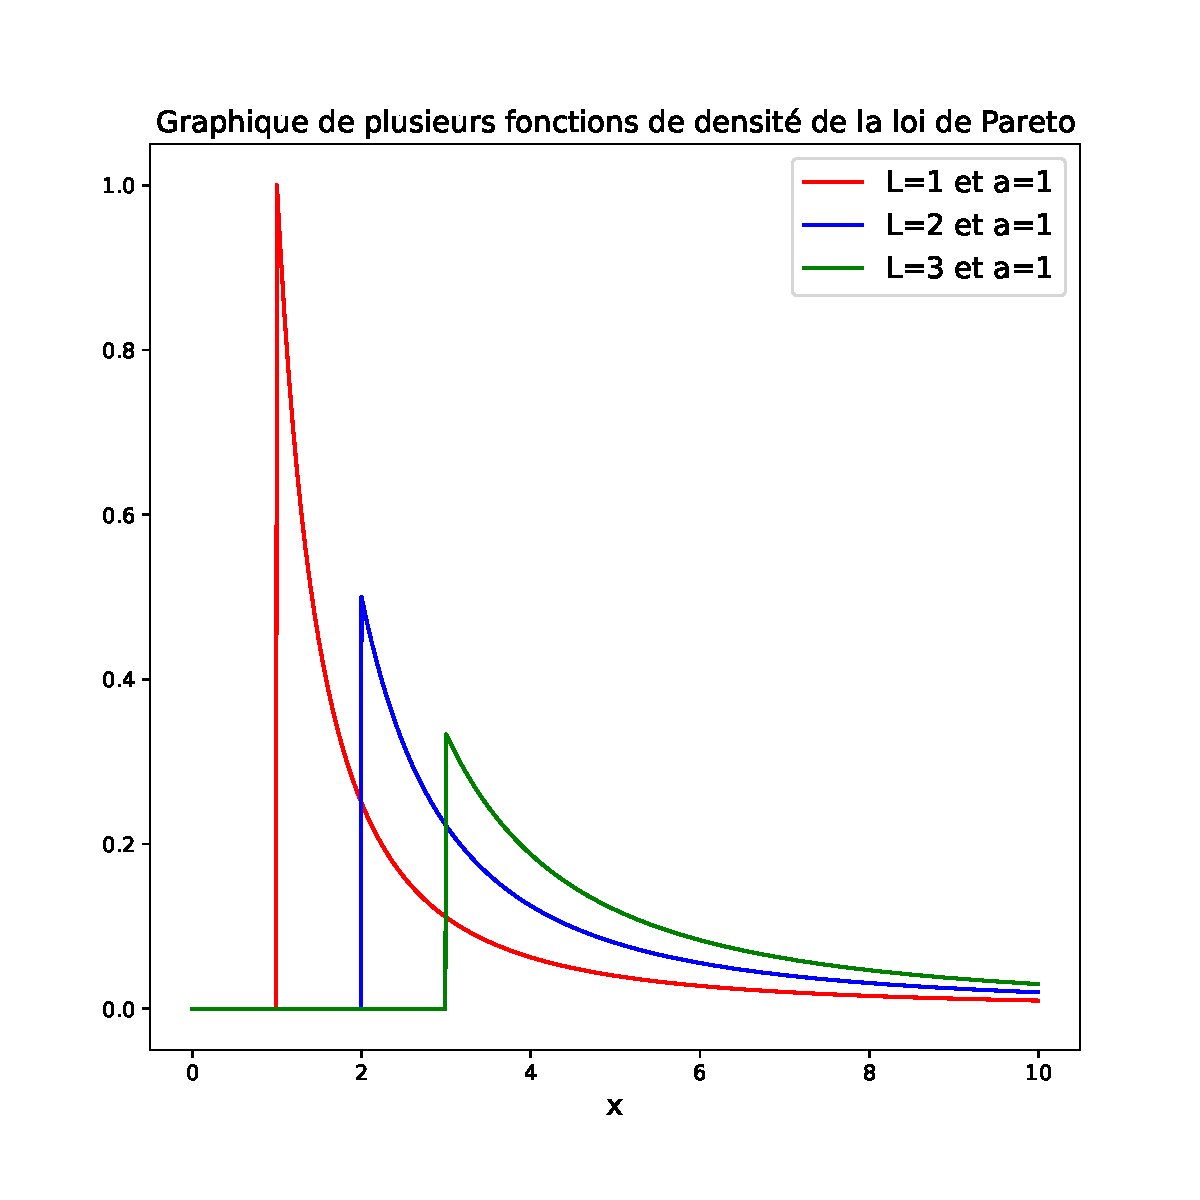
\includegraphics[scale=0.25]{graphiques_Pareto.pdf}
\end{center}
\end{figure}


\end{frame}





\end{document}
